\documentclass[10pt]{article}
\usepackage[polish]{babel}
\usepackage[utf8]{inputenc}
\usepackage[T1]{fontenc}
\usepackage{amsmath}
\usepackage{amsfonts}
\usepackage{amssymb}
\usepackage[version=4]{mhchem}
\usepackage{stmaryrd}
\usepackage{graphicx}
\usepackage[export]{adjustbox}
\graphicspath{ {./images/} }

\begin{document}
\begin{enumerate}
  \item Do przedziału w pociągu, w którym jest osiem miejsc, cztery na jednej kanapie i cztery na drugiej, wsiada 6 osób, w tym Kowalski i Nowak, i losowo zajmują miejsca. Jakie jest prawdopodobieństwo, że Kowalski i Nowak usiądą naprzeciwko siebie?
  \item Dwunastu chłopców, wśród których są Kowalski i Nowak losowo dzielimy na trzy równoliczne drużyny. Jakie jest prawdopodobieństwo, że Kowalski i Nowak znajdą się w tej samej drużynie?
  \item Prosta \(k\) jest styczna do okręgu o w punkcie A. Odcinek CD jest cięciwą okręgu o równoległą do prostej \(k\). Styczna do okręgu o w punkcie D przecina prostą \(k\) w punkcie B. Odcinek BC przecina okrąg o w punkcie E. Dowieść, że prosta DE dzieli odcinek \(A B\) na dwie równe części.\\
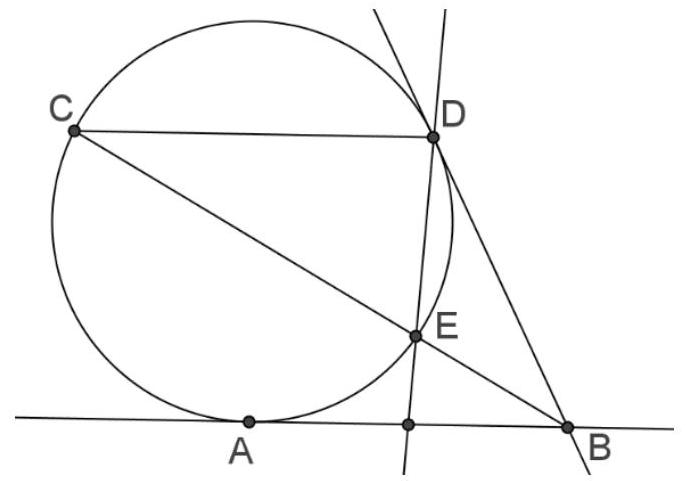
\includegraphics[max width=\textwidth, center]{2024_11_21_2623276ecdaf945c4cb3g-1}
\end{enumerate}

\end{document}